\documentclass[aspectratio=169, table]{beamer}

\usepackage[utf8]{inputenc}
\usepackage{listings} 

\usetheme{Pradita}

\subtitle{IF140303-Web Application Development}

\title{\LARGE{Session-05:\\ Avatar Generator in Elixir}
	\vspace{20pt}}
\date[Serial]{\scriptsize {PRU/SPMI/FR-BM-18/0222}}
\author[Pradita]{\small{\textbf{Alfa Yohannis}}}

\lstdefinelanguage{Elixir} {
	keywords={def, defmodule, do, end, for, if, else, true, false},
	basicstyle=\ttfamily\small,
	keywordstyle=\color{blue}\bfseries,
	ndkeywords={@moduledoc, iex, Enum, @doc},
	ndkeywordstyle=\color{purple}\bfseries,
	sensitive=true,
	commentstyle=\color{gray},
	stringstyle=\color{red},
	numbers=left,
	numberstyle=\tiny\color{gray},
	breaklines=true,
	frame=lines,
	backgroundcolor=\color{lightgray!10},
	tabsize=2,
	comment=[l]{\#},
	morecomment=[s]{/*}{*/},
	commentstyle=\color{gray}\ttfamily,
	stringstyle=\color{purple}\ttfamily,
	showstringspaces=false
}

\begin{document}
	
	\frame{\titlepage}
	
	
		\begin{frame}
			\frametitle{Avatar Generator}
			\begin{center}
				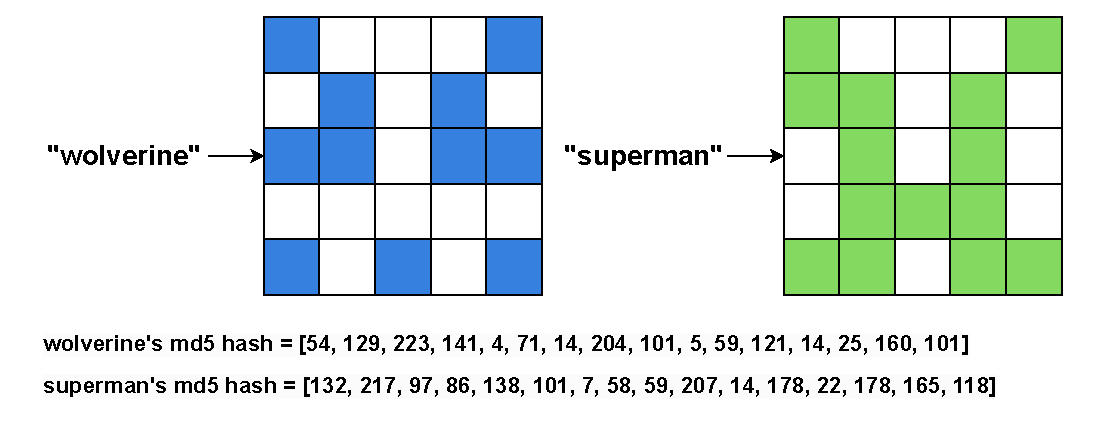
\includegraphics[width=1\textwidth]{../../assets/avatar-example.pdf}
			\end{center}
		\end{frame}
	

	\begin{frame}
		\frametitle{Avatar Pipeline}
		\vspace{20pt}
		\begin{center}
			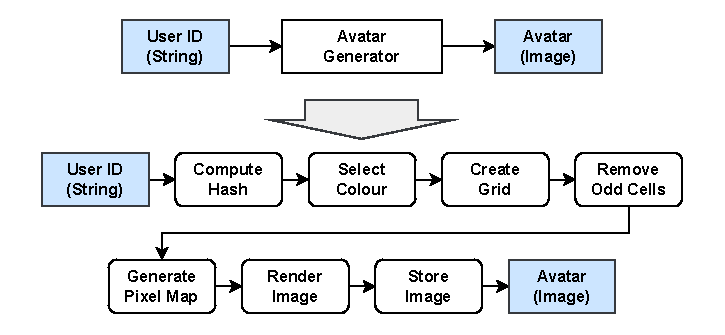
\includegraphics[width=1\textwidth]{../../assets/avatar-pipeline.pdf}
		\end{center}
	\end{frame}

	\begin{frame}
		\frametitle{Avatar Computation}
		\vspace{20pt}
		\begin{center}
			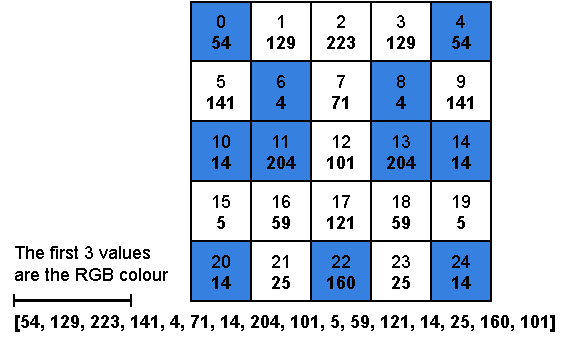
\includegraphics[width=0.9\textwidth]{../../assets/avatar-computation.pdf}
		\end{center}
	\end{frame}

	
	\begin{frame}
		\frametitle{Avatar Overview}
		\begin{itemize}
			\item The avatar is represented by a 5x5 grid, with each cell being 50x50 pixels.
			\item The grid is symmetrical, where the middle column acts as a mirror for the left and right sides.
			\item This grid-based avatar is a unique, visual representation of input data, often used as a personal identifier.
		\end{itemize}
	\end{frame}
	
	\begin{frame}
		\frametitle{Project: Avatar Generator App}
		\begin{itemize}
			\item We will create an avatar generator that produces a consistent avatar for the same input string.
			\item The avatar will be a visual identifier generated uniquely from the string.
			\item The project will be built step-by-step, with each step implemented through specific functions.
		\end{itemize}
	\end{frame}
	
	\begin{frame}
		\frametitle{Avatar Generator Workflow}
		\begin{enumerate}
			\item Accept an input string.
			\item Generate an MD5 hash from the string.
			\item Convert the hash into a list of numbers.
			\item Choose a color based on the hash values.
			\item Create a symmetrical grid based on these numbers.
			\item Convert the grid into an image.
			\item Save the generated image as a PNG file.
		\end{enumerate}
	\end{frame}
	
	\begin{frame}[fragile]
		\frametitle{Hashing the Input String}
		\begin{lstlisting}[language=Elixir]
			iex> hash = :crypto.hash(:sha256, "banana")
			<<180, 147, 212, 131, 100, 175, 228, 77, 17, 192, 22, 92, 244, 112, 164, 22, 77,
			30, 38, 9, 145, 30, 249, 152, 190, 134, 141, 70, 173, 227, 222, 78>>
			
			iex> :binary.bin_to_list(hash)
			[180, 147, 212, 131, 100, 175, 228, 77, 17, 192, 22, 92, 244, 112, 164, 22, 77,
			30, 38, 9, 145, 30, 249, 152, 190, 134, 141, 70, 173, 227, 222, 78]
		\end{lstlisting}
		\begin{itemize}
			\item We compute the MD5 hash of the input string using \texttt{:crypto.hash/2}.
			\item The binary hash is then converted into a list of integers using \texttt{:binary.bin\_to\_list/1}.
		\end{itemize}
	\end{frame}
	
	\begin{frame}[fragile]
		\frametitle{Starting the Implementation}
		\begin{lstlisting}[language=Elixir]
			def compute_hash(input) do
			hash = :crypto.hash(:sha256, input)
			|> :binary.bin_to_list
			
			%Avatar.Image{hash: hash}
		\end{lstlisting}
		\begin{itemize}
			\item We start by defining the \texttt{hash\_input/1} function.
			\item This function takes a string, computes its hash, and returns a structure with the hash.
		\end{itemize}
	\end{frame}
	
	\begin{frame}[fragile]
		\frametitle{Running the Code in IEx}
		\begin{itemize}
			\item To execute the code, we use IEx (Interactive Elixir) as follows:
		\end{itemize}
		\begin{lstlisting}[language=Elixir]
			iex> AvatarGenerator.generate("banana")
			hash: [180, 147, 212, 131, 100, 175, 228, 77, 17, 192, 22, 92, 244, 112, 164,
			22, 77, 30, 38, 9, 145, 30, 249, 152, 190, 134, 141, 70, 173, 227, 222, 78],
		\end{lstlisting}
		\begin{itemize}
			\item This command will generate an avatar based on the string \texttt{"banana"}.
		\end{itemize}
	\end{frame}
	
	\begin{frame}
		\frametitle{Generating RGB Values}
		\begin{itemize}
			\item The first three values from the hash list are used to generate an RGB color.
			\item This color will be applied to specific cells in the grid.
		\end{itemize}
	\end{frame}
	
	\begin{frame}
		\frametitle{Grid Pattern}
		\begin{itemize}
			\item The grid pattern for the avatar follows this symmetry:
		\end{itemize}
		\begin{center}
			\texttt{1 2 3 2 1} \\
			\texttt{4 5 6 5 4} \\
			\texttt{7 8 9 8 7} \\
			\texttt{10 11 12 11 10} \\
			\texttt{13 14 15 14 13}
		\end{center}
		\begin{itemize}
			\item All even-numbered cells in the grid will be filled with the generated RGB color.
		\end{itemize}
	\end{frame}
	
	\begin{frame}
		\frametitle{Summary}
		\begin{itemize}
			\item We discussed the Avatar Generator project and its workflow.
			\item We covered how to hash a string and use the hash to determine the avatar's color.
			\item We also explained how the grid is formed and how colors are applied based on hash values.
		\end{itemize}
	\end{frame}
	
\end{document}
